L'idée dans la formule de cette nouvelle couche $\mathcal{S}$MorphTanh dérivée de $\mathcal{S}$Morph est simplement d'ajouter un facteur multiplicateur devant les valeurs du noyau $w$ dans la formule de $\mathcal{S}$Morph (\ref{SMorph}), facteur qui puisse être le reflet d'une transition lisse entre le signe $+$ et $-$ lors du passage de $\alpha$ d'un signe positive à un signe négatif, et inversement. Ce facteur est ici défini par la tangente hyperbolique de $\alpha$ : $\tanh{(\alpha)}$. \\

La formule de $\mathcal{S}$MorphNetTanh, pour une image $f: I \subseteq \mathbb{Z}^2 \rightarrow \mathbb{R}$ et un noyau de couche $w: W \subseteq \mathbb{Z}^2 \rightarrow \mathbb{R}$, et avec $\alpha \in \mathbb{R}$, est ainsi définie pour tout $x \in I$ par :

\begin{equation}
    \pmb{\mathcal{S}}\textbf{MorphTanh} (f,w,\alpha)(x) = \frac{\sum_{y \in \breve{W}_x} (f(y) + \tanh{(\alpha)} w(x-y))e^{\alpha (f(y) + \tanh{(\alpha)} w(x-y))}}{\sum_{y \in \breve{W}_x} e^{\alpha (f(y) + \tanh{(\alpha)} w(x-y))}}
    \label{SMorphTanh}
\end{equation}

\vspace{3.0mm}
\noindent Le facteur $\tanh{(\alpha)}$ permet bien, à la fois, d'ajuster le signe de $w$ dans la formulation asymptotique de $\mathcal{S}$Morph, et de lisser l'espace de la \textit{loss} pour $\alpha$ au voisinage de $0$, en réduisant l'impact des variations des poids $\text{w}_i$ dans la formule de $\mathcal{S}$MorphTanh, grâce à ce $\tanh{(\alpha)}$ devant $w$, qui est proche de $0$ quand $\alpha$ est au voisinage de $0$. \\

%figure
\vspace{-1.5mm}
\begin{figure}[ht]
  \begin{center}
      \subfigure[$(\text{w},\alpha) \mapsto \text{w}$]{
          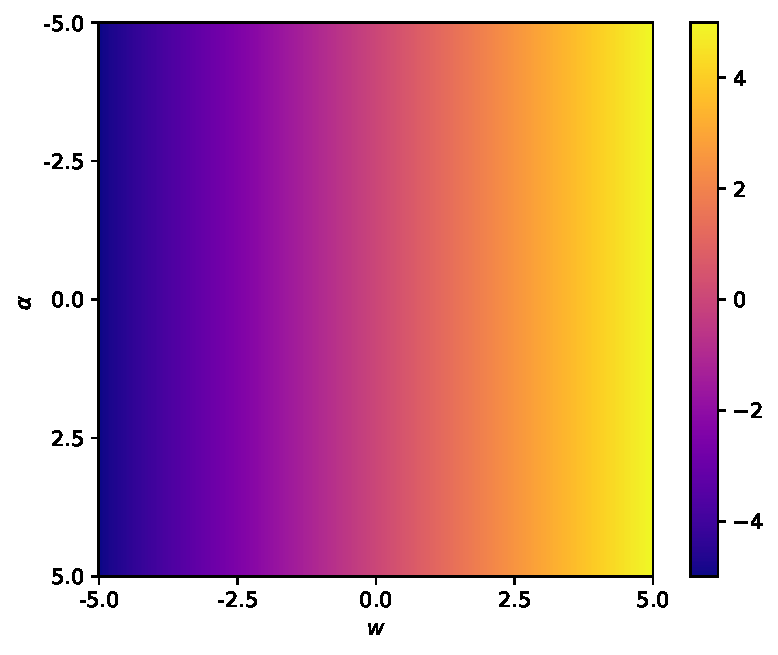
\includegraphics[width=0.30\textwidth]{parts/3-contributions/A-reseaux_smorphTANH/figures/image_wa_s.pdf}
          \label{fig:suh1}}
      \hspace{12.0mm}
      \subfigure[$(\text{w},\alpha) \mapsto \tanh{(\alpha)} \times \text{w}$]{
          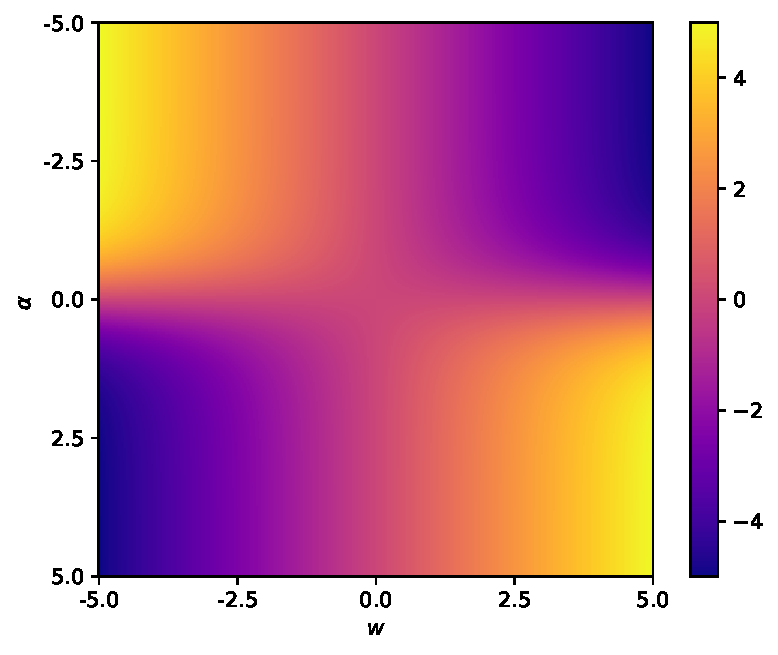
\includegraphics[width=0.30\linewidth]{parts/3-contributions/A-reseaux_smorphTANH/figures/image_wa_sh.pdf}
          \label{fig:suh2}}
    \caption{ \centering Carte de la fonction $(\text{w},\alpha) \mapsto \text{w}$ représentant $\mathcal{S}$MorphNet (gauche \ref{fig:suh1}) et de la fonction $(\text{w},\alpha) \mapsto \tanh{(\alpha)} \times \text{w}$ représentant $\mathcal{S}$MorphNetTanh (droite \ref{fig:suh2}).}
    \label{fig:espace_s_vs_sh}
  \end{center}
\end{figure}

\vspace{-4.0mm}
\noindent La figure \ref{fig:espace_s_vs_sh} ci-dessus montre l'évolution des valeurs (en couleurs) de la fonction $(\text{w},\alpha) \mapsto \tanh{(\alpha)} \times \text{w}$ en fonction de w (en abscisse) et $\alpha$(en ordonnée). La carte \ref{fig:suh1} reflète le comportement de $\mathcal{S}$Morph sur une image $f$ nulle et avec un seul poids w du noyau $w$, et la carte \ref{fig:suh2} reflète celui de $\mathcal{S}$MorphTanh. On remarque bien sur \ref{fig:suh1} le passage continue d'un signe positif à un signe négatif de $\alpha$ en ordonnée, ainsi que le lissage de la fonction au voisinage de $\alpha \approx 0$ selon le poids w en abscisse. \\
%\noindent La figure ci-dessus montre l'évolution des valeurs de la fonction $(\text{w},\alpha) \mapsto \tanh{(\alpha)} \times \text{w}$ avec le passage continue d'un signe positif à un signe négatif de $\alpha$ en ordonnée. Il montre également le lissage, au voisinage de $\alpha \approx 0$, de la fonction $\textit{w} \mapsto \tanh{(\alpha)} \times \text{w}$ selon le poids \textit{w} sur l'axe des abscisses. \\

\vspace{-1.6mm}
\noindent On obtient bien l'image $f \ominus \breve{w}$ quand $\alpha \rightarrow -\infty$, et toujours $f \oplus w$ quand $\alpha \rightarrow +\infty$.
